\subsection{Handwritten Gauss Newton Method}

Next we use a simple example to illustrate how to solve the least squares problem. We will demonstrate how to handwrite the Gauss-Newton method and then how to use the optimization library to solve this problem. For the same problem, these implementations will achieve the same result because their core algorithms are the same.

Consider a curve that satisfies the following equation:

\[
y = \exp( ax^2 + bx + c ) + w,
\]

Where $a,b,c$ are the parameters of the curve, and $w$ is Gaussian noise, satisfying $w \sim (0, \sigma^2)$. We deliberately chose such a nonlinear model so that the problem is not too simple. Now, suppose we have $N$ observation data points for $x,y$, and we want to find the parameters of the curve based on these data points. Then, the following least squares problem can be solved to estimate the curve parameters:

\begin{equation}
\min \limits_{a,b,c} \frac{1}{2}\sum\limits_{i = 1}^N {{{\left\| {{y_i} - \exp \left( {ax_i^2 + bx_i + c} \right)} \right\|}^2}} .
\end{equation}

Note that in this question, the variables to be estimated are $a,b,c$ instead of $x$. In our program, we first generate the true value of $x, y$ according to the model, and then add the Gaussian distribution noise to the true value. Subsequently, the Gauss-Newton method is used to fit the parametric model from the noisy data. The definition error is:

\begin{equation}
e_i = y_i - \exp \left( {ax_i^2 + bx_i + c} \right),
\end{equation}

Then we can find the derivative of each error term for the state variable:

\begin{equation}
\begin{aligned}
\frac{{\partial {e_i}}}{{\partial a}} &=  - x_i^2\exp \left( {ax_i^2 + b{x_i} + c} \right)\\
\frac{{\partial e_i}}{{\partial b}} &=  - {x_i}\exp \left( {ax_i^2 + b{x_i} + c} \right)\\
\frac{{\partial {e_i}}}{{\partial c}} &=  - \exp \left( {ax_i^2 + b{x_i} + c} \right)
\end{aligned}
\end{equation}

Then $\bm{J}_i = \left[\frac{{\partial {e_i}}}{{\partial a}},\frac{{\partial {e_i}}}{{\partial b}}, \frac{{\partial {e_i}}}{{\partial c}} \right]^\mathrm{T}$, the incremental equation for the Gauss-Newton method is:

\begin{equation}
\left(\sum\limits_{i = 1}^{100} {\bm{J}_i{(\sigma^2)^{ - 1}}{\bm{J}_i}}^\mathrm{T} \right) \Delta \bm{x}_k = \sum\limits_{i = 1}^{100} { - {\bm{J}_i}{(\sigma^2)^{ - 1}}{e_i}},
\end{equation}

Of course, we can also choose to put all the $\bm{J}_i$ in a column and write the equation as a matrix, but its meaning is consistent with the summation form. The code below demonstrates how this process works.

\begin{lstlisting}[language=sh,caption=slambook2/ch6/gaussNewton.cpp]
#include <iostream>
#include <opencv2/opencv.hpp>
#include <Eigen/Core>
#include <Eigen/Dense>

Using namespace std;
Using namespace Eigen;

Int main(int argc, char **argv) {
Double ar = 1.0, br = 2.0, cr = 1.0; // true parameter value
Double ae = 2.0, be = -1.0, ce = 5.0; // estimate parameter value
Int N = 100; // data points
Double w_sigma = 1.0; // noise sigma value
Double inv_sigma = 1.0 / w_sigma;
Cv::RNG rng; // OpenCV random number generator

Vector<double> x_data, y_data; // data
For (int i = 0; i < N; i++) {
Double x = i / 100.0;
X_data.push_back(x);
Y_data.push_back(exp(ar * x * x + br * x + cr) + rng.gaussian(w_sigma * w_sigma));
}

// Start Gauss-Newton iteration
Int iterations = 100; // number of iterations
Double cost = 0, lastCost = 0; // cost of this iteration and cost of the last iteration

Chrono::steady_clock::time_point t1 = chrono::steady_clock::now();
For (int iter = 0; iter < iterations; iter++) {

Matrix3d H = Matrix3d::Zero(); // Hessian = J^TW^{-1} J in Gauss-Newton
Vector3d b = Vector3d::Zero(); // bias
Cost = 0;

For (int i = 0; i < N; i++) {
Double xi = x_data[i], yi = y_data[i]; // ith data point
Double error = yi - exp(ae * xi * xi + be * xi + ce);
Vector3d J; // Jacobian matrix
J[0] = -xi * xi * exp(ae * xi * xi + be * xi + ce); // de/da
J[1] = -xi * exp(ae * xi * xi + be * xi + ce); // de/db
J[2] = -exp(ae * xi * xi + be * xi + ce); // de/dc

H += inv_sigma * inv_sigma * J * J.transpose();
b += -inv_sigma * inv_sigma * error * J;

Cost += error * error;
}

/ / Solve the linear equation Hx = b
Vector3d dx = H.ldlt().solve(b);
If (isnan(dx[0])) {
Cout << "result is nan!" << endl;
Break;
}

If (iter > 0 && cost >= lastCost) {
Cout << "cost: " << cost << ">= last cost: " << lastCost << ", break." << endl;
Break;
}

Ae += dx[0];
Be += dx[1];
Ce += dx[2];

lastCost = cost;

Cout << "total cost: " << cost << ", \t\tupdate: " << dx.transpose() <<
"\t\testimated params: " << ae << "," << be << "," << ce << endl;
}

Chrono::steady_clock::time_point t2 = chrono::steady_clock::now();
Chrono::duration<double> time_used = chrono::duration_cast<chrono::duration<double>>(t2 - t1);
Cout << "solve time cost = " << time_used.count() << " seconds. " << endl;
Cout << "estimated abc = " << ae << ", " << be << ", " << ce << endl;
Return 0;
}
\end{lstlisting}

In this example, we demonstrate how to iteratively optimize a simple fitting problem. It's easy to see the entire optimization process with your own handwritten code. The program outputs the target function value and update amount for each iteration of the iteration, as follows:

\begin{lstlisting}[language=sh,caption=Terminal output:]
/home/xiang/Code/slambook2/ch6/cmake-build-debug/gaussNewton
total cost: 3.19575e+06, 		update: 0.0455771  0.078164 -0.985329		estimated params: 2.04558,-0.921836,4.01467
total cost: 376785, 		update:  0.065762  0.224972 -0.962521		estimated params: 2.11134,-0.696864,3.05215
total cost: 35673.6, 		update: -0.0670241   0.617616  -0.907497		estimated params: 2.04432,-0.0792484,2.14465
total cost: 2195.01, 		update: -0.522767   1.19192 -0.756452		estimated params: 1.52155,1.11267,1.3882
total cost: 174.853, 		update: -0.537502  0.909933 -0.386395		estimated params: 0.984045,2.0226,1.00181
total cost: 102.78, 		update: -0.0919666   0.147331 -0.0573675		estimated params: 0.892079,2.16994,0.944438
total cost: 101.937, 		update: -0.00117081  0.00196749 -0.00081055		estimated params: 0.890908,2.1719,0.943628
total cost: 101.937, 		update:   3.4312e-06 -4.28555e-06  1.08348e-06		estimated params: 0.890912,2.1719,0.943629
total cost: 101.937, 		update: -2.01204e-08  2.68928e-08 -7.86602e-09		estimated params: 0.890912,2.1719,0.943629
cost: 101.937>= last cost: 101.937, break.
solve time cost = 0.000212903 seconds.
estimated abc = 0.890912, 2.1719, 0.943629
\end{lstlisting}

The objective function that is easy to see the whole problem approaches convergence after 9 iterations, and the update amount approaches zero. The final estimated value is close to the true value, as shown in \autoref{fig:ceres-fitting}. On my machine (my CPU is i7-8700), the optimization takes about 0.2 milliseconds. Below we try to use the optimization library to accomplish the same task.

\begin{figure}[!ht]
	\centering
	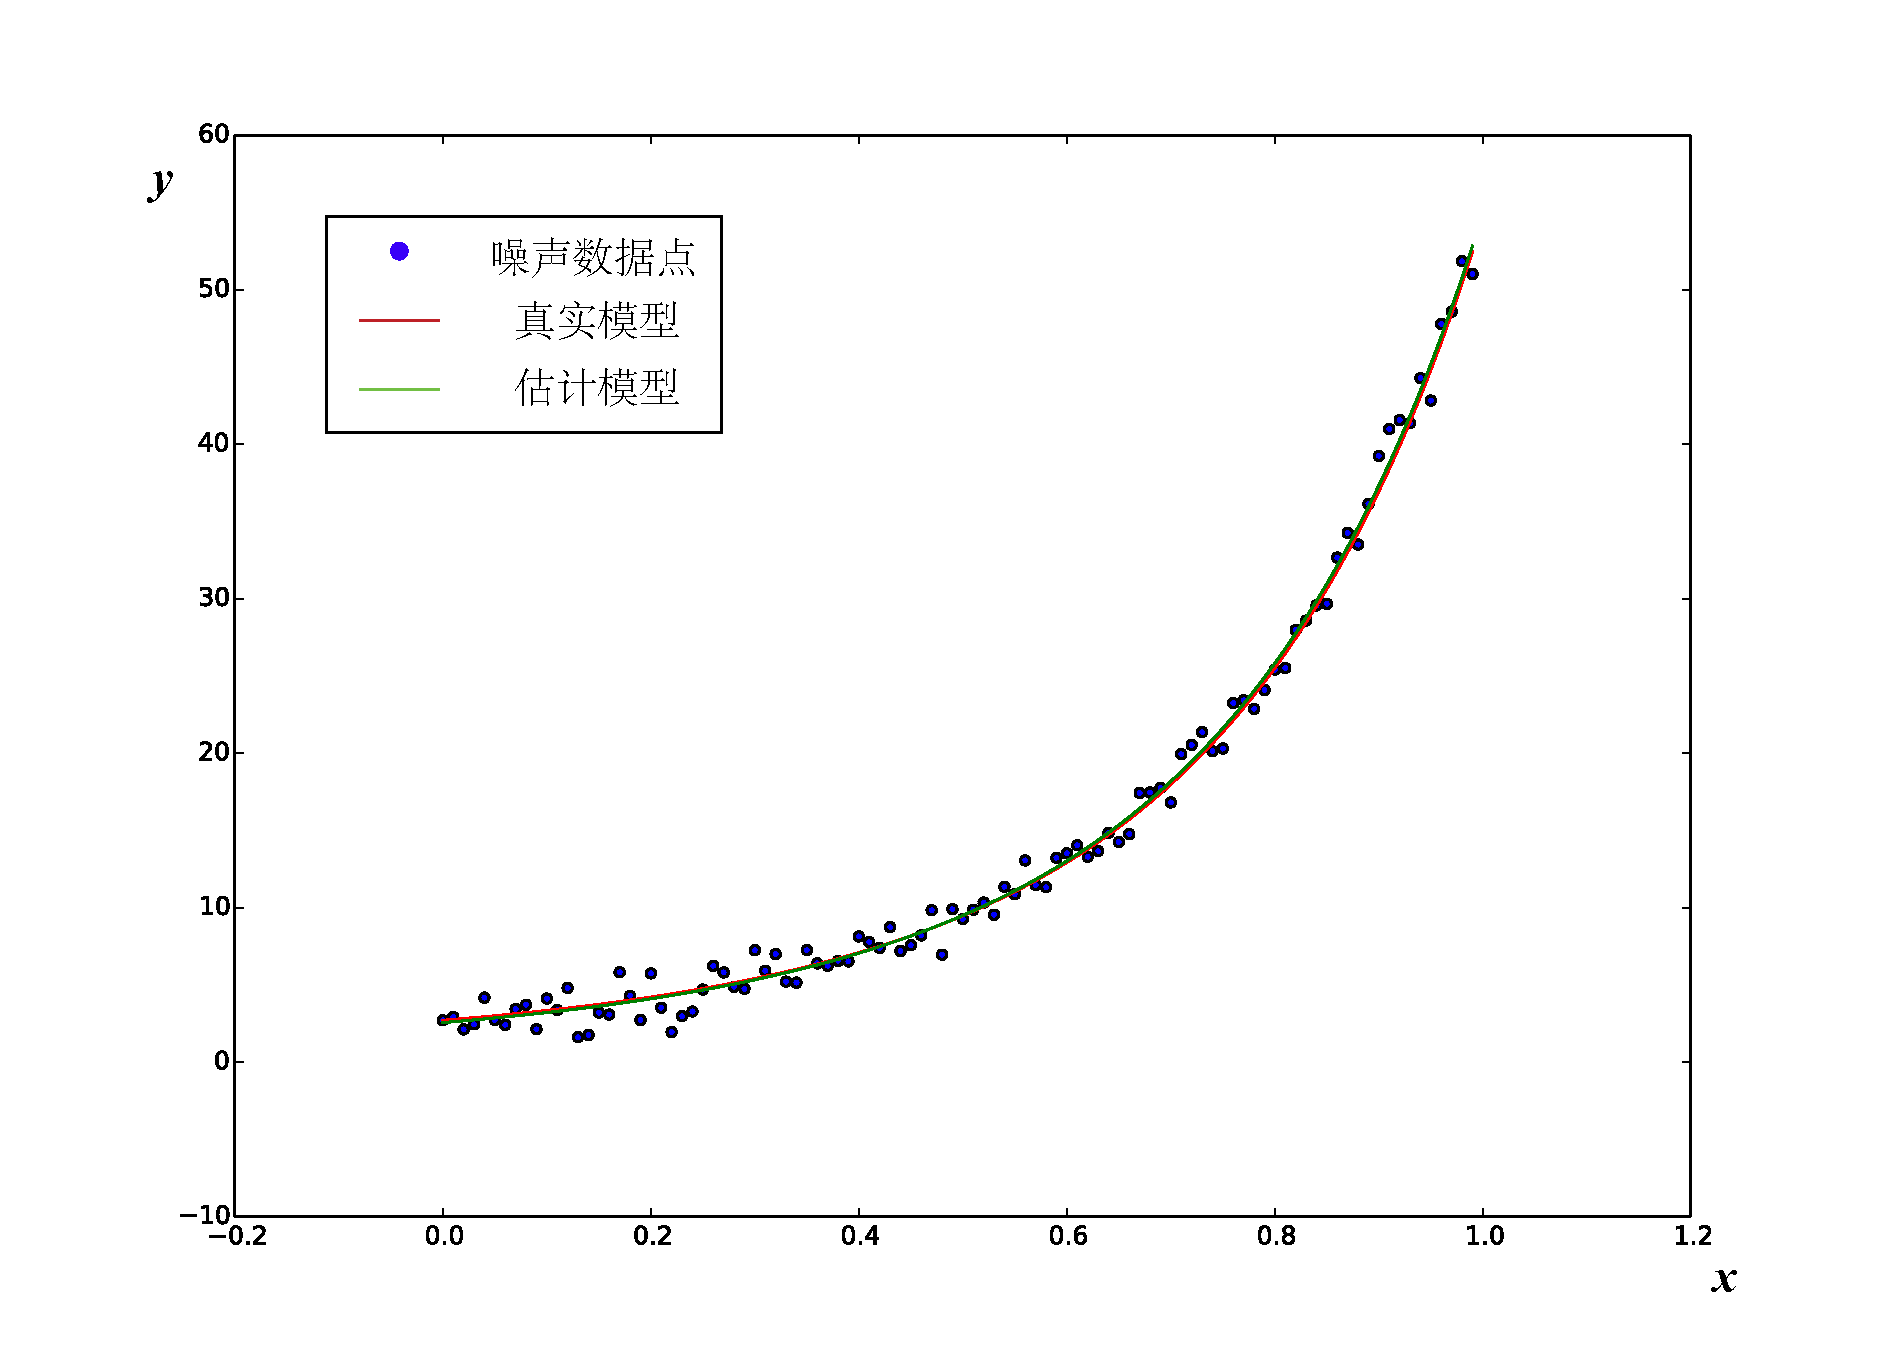
\includegraphics[width=0.8\textwidth]{chapter06/optimization/ceresFitting.pdf}
	\caption{The result of curve fitting when noise $\sigma=1$. The real model is very close to the estimated model. }
	\label{fig:ceres-fitting}
\end{figure}
